% Définition du Process Hitting + sortes coopératives

%san presentation
\begin{comment}
\begin{frame}
\frametitle{Biological networks modelling}
\begin{tikzpicture}
\node (brn) at (0,5) {\begin{tikzpicture}[auto,scale=0.9] 
                                                 \path[use as bounding box] (-0.7,-0.3) rectangle (2.5,2);

                                                              \node[qgre,scale=0.8] (a) at (0,2) {a};
                                                              \node[mod,scale=0.8] (i) at (1,1) {i};
                                                              \node[qgre,scale=0.8] (b) at (0,0) {b};
                                                              \node[qgre,scale=0.8] (c) at (2,1) {c};
                                                              \path
                                                                (a) edge[inh,scale=0.1] (i)
                                                                (b) edge[act,scale=0.1] (i)
                                                                (i) edge[st,scale=0.1]  (c);
                                                              
                                                 \end{tikzpicture}};
\node[scale=0.6] (an) at (7,5) {\begin{tikzpicture}
\exandef
\end{tikzpicture}};
\node[scale=0.6] (sg) at (2,1) {
\begin{tikzpicture}[line join=bevel,font=\LARGE]
%%
  \node (6) at (405.0bp,18.0bp) [reach,nd4] {$\langle a_2,b_1,c_0\rangle$};
  \node (2) at (405.0bp,90.0bp) [reach,nd3] {$\langle a_2,b_0,c_0\rangle$};
  \node (1) at (570.0bp,90.0bp) [reach,nd1] {$\langle a_1,b_0,c_0\rangle$};
  \node (0) at (469.0bp,162.0bp) [reach,nd0] {$s_0 = \langle a_0,b_0,c_0\rangle$};
  \node (4) at (469.0bp,234.0bp) [reach,nd5] {$\langle a_0,b_1,c_0\rangle$};
 
 
  \draw [->,arc3] (0) ..controls (445.65bp,135.46bp) and (435.95bp,124.86bp)  .. (2);
  \draw [->,arc5] (0) ..controls (475.71bp,188.03bp) and (475.94bp,197.36bp)  .. (4);
  \draw [->,arc4] (2) ..controls (405.0bp,63.983bp) and (405.0bp,54.712bp)  .. (6);
  \draw [->,arc1] (0) ..controls (499.93bp,134.79bp) and (517.41bp,122.58bp)  .. (1);
  \draw [->,arc2] (1) ..controls (539.0bp,117.26bp) and (521.52bp,129.47bp)  .. (0);
  \draw [->,arc5] (4) ..controls (462.3bp,208.35bp) and (462.06bp,199.03bp)  .. (0);
 
%
\end{tikzpicture}

};
\path 
(brn) edge[->,line width=8pt, color=lightgray] (an)
(an) edge[->,line width=8pt, color=lightgray,bend left] (sg)
;

\end{tikzpicture}
\end{frame}


\begin{frame}
  \frametitle{Réseaux d'automates stochastiques}
  
\begin{columns}
\begin{column}{0.6\textwidth}

% Automate sans les rates
\only<1->{
\tikzstyle{tick}=[densely dotted]
\tikzstyle{hit}=[->,>=angle 45]
\tikzstyle{selfhit}=[min distance=30pt,curve to]
\tikzstyle{bounce}=[densely dotted,>=stealth',->]
\tikzstyle{hlhit}=[very thick]
\begin{center}\scalebox{\scaleex}{
\begin{tikzpicture}
\exandef
\end{tikzpicture}
}\end{center}
}
\end{column}

\begin{column}{0.4\textwidth}
\begin{figure}[p]
\centering

\scalebox{0.4}{

\only<1->{
\tikzstyle{arc0}=[->]
\tikzstyle{nd0}=[]
\tikzstyle{arc1}=[->]
\tikzstyle{nd1}=[]
\tikzstyle{arc2}=[->]
\tikzstyle{nd2}=[]
\tikzstyle{arc3}=[->]
\tikzstyle{nd3}=[]
\tikzstyle{arc4}=[->]
\tikzstyle{nd4}=[]
\tikzstyle{arc5}=[->]
\tikzstyle{nd5}=[]

\begin{tikzpicture}[line join=bevel,font=\LARGE]
%%
  \node (6) at (405.0bp,18.0bp) [reach,nd4] {$\langle a_2,b_1,c_0\rangle$};
  \node (2) at (405.0bp,90.0bp) [reach,nd3] {$\langle a_2,b_0,c_0\rangle$};
  \node (1) at (570.0bp,90.0bp) [reach,nd1] {$\langle a_1,b_0,c_0\rangle$};
  \node (0) at (469.0bp,162.0bp) [reach,nd0] {$s_0 = \langle a_0,b_0,c_0\rangle$};
  \node (4) at (469.0bp,234.0bp) [reach,nd5] {$\langle a_0,b_1,c_0\rangle$};
 
 
  \draw [->,arc3] (0) ..controls (445.65bp,135.46bp) and (435.95bp,124.86bp)  .. (2);
  \draw [->,arc5] (0) ..controls (475.71bp,188.03bp) and (475.94bp,197.36bp)  .. (4);
  \draw [->,arc4] (2) ..controls (405.0bp,63.983bp) and (405.0bp,54.712bp)  .. (6);
  \draw [->,arc1] (0) ..controls (499.93bp,134.79bp) and (517.41bp,122.58bp)  .. (1);
  \draw [->,arc2] (1) ..controls (539.0bp,117.26bp) and (521.52bp,129.47bp)  .. (0);
  \draw [->,arc5] (4) ..controls (462.3bp,208.35bp) and (462.06bp,199.03bp)  .. (0);
 
%
\end{tikzpicture}


}
}

\end{figure}

\end{column}
\end{columns}

\begin{liste}
  \item \tval{Automates}: composants \qex{$a$, $b$, $c$}.
  \item \tval{\'Etats locaux}: niveaux d'expression \qex{$c_0$, $c_1$, $c_2$}.
  \item \tval{States}: sets of active local states%
  \only<1->{\qex{$\PHetat{a_2, b_1, c_0}$}}
  \item \tval{Transitions}: dynamique \qex{\only<1->{$t_1 = \trans{a_0}{a_1}{b_0}$}, \only<1->{$t_2 = \trans{a_1}{a_0}{}$}, \only<1->{$t_3 = \trans{a_0}{a_2}{b_0,c_0}$}, \only<1->{$t_4 = \trans{b_0}{b_1}{}$}}
\end{liste}
\end{frame}
\end{comment}

\begin{frame}
  \frametitle{Réseaux d'automates stochastiques}
  %\framesubtitle{\tcite{Paulev\'e et al. 2012}}
\begin{columns}
\begin{column}{0.6\textwidth}

% Automate avec les rates
\only<1->{
\tikzstyle{tick}=[densely dotted]
\tikzstyle{hit}=[->,>=angle 45]
\tikzstyle{selfhit}=[min distance=30pt,curve to]
\tikzstyle{bounce}=[densely dotted,>=stealth',->]
\tikzstyle{hlhit}=[very thick]
\begin{center}\scalebox{\scaleex}{
\begin{tikzpicture}
\exsandef
\end{tikzpicture}
}\end{center}
}
\end{column}

\begin{column}{0.4\textwidth}
\begin{figure}[p]
\centering

\scalebox{0.4}{

\only<1->{
\tikzstyle{arc0}=[->]
\tikzstyle{nd0}=[]
\tikzstyle{arc1}=[->]
\tikzstyle{nd1}=[]
\tikzstyle{arc2}=[->]
\tikzstyle{nd2}=[]
\tikzstyle{arc3}=[->]
\tikzstyle{nd3}=[]
\tikzstyle{arc4}=[->]
\tikzstyle{nd4}=[]
\tikzstyle{arc5}=[->]
\tikzstyle{nd5}=[]

\begin{tikzpicture}[line join=bevel,font=\LARGE]
%%
  \node (6) at (405.0bp,18.0bp) [reach,nd4] {$\langle a_2,b_1,c_0\rangle$};
  \node (2) at (405.0bp,90.0bp) [reach,nd3] {$\langle a_2,b_0,c_0\rangle$};
  \node (1) at (570.0bp,90.0bp) [reach,nd1] {$\langle a_1,b_0,c_0\rangle$};
  \node (0) at (469.0bp,162.0bp) [reach,nd0] {$s_0 = \langle a_0,b_0,c_0\rangle$};
  \node (4) at (469.0bp,234.0bp) [reach,nd5] {$\langle a_0,b_1,c_0\rangle$};
 
 
  \draw [->,arc3] (0) ..controls (445.65bp,135.46bp) and (435.95bp,124.86bp)  .. node[auto] {$\mathbf{\color{Maroon} 2}$}(2) ;
  \draw [->,arc5] (0) ..controls (475.71bp,188.03bp) and (475.94bp,197.36bp)  .. node[right] {$\mathbf{\color{Maroon} 3}$}(4) ;
  \draw [->,arc4] (2) ..controls (405.0bp,63.983bp) and (405.0bp,54.712bp)  .. node[auto] {$\mathbf{\color{Maroon} 3}$}(6) ;
  \draw [->,arc1] (0) ..controls (499.93bp,134.79bp) and (517.41bp,122.58bp)  .. node[auto] {$\mathbf{\color{Maroon} 1}$}(1) ;
  \draw [->,arc2] (1) ..controls (539.0bp,117.26bp) and (521.52bp,129.47bp)  .. node[auto] {$\mathbf{\color{Maroon} 2}$}(0) ;
  \draw [->,arc5] (4) ..controls (462.3bp,208.35bp) and (462.06bp,199.03bp)  .. node[left] {$\mathbf{\color{Maroon} 1}$}(0) ;
 
%
\end{tikzpicture}


}
}

\end{figure}

\end{column}
\end{columns}

\begin{liste}
  \item \tval{Automates}: composants \qex{$a$, $b$, $c$}
  \item \tval{\'Etats locaux}: niveaux d'expression \qex{$c_0$, $c_1$, $c_2$}
  \item \tval{\'Etat}: ensemble des états locaux actifs%
  \only<1->{\qex{$\PHetat{a_2, b_1, c_0}$}}
  \item \tval{Transitions}: dynamique \qex{\only<1->{$t_1 = \trans{a_0}{a_1}{b_0,\mathbf{\color{Maroon} 2}}$}, \only<1->{$t_2 = \trans{a_1}{a_0}{\mathbf{\color{Maroon} 1}}$}, \only<1->{$t_3 = \trans{a_0}{a_2}{b_0,c_0,\mathbf{\color{Maroon} 2}}$}, \only<1->{$t_4 = \trans{b_0}{b_1}{\mathbf{\color{Maroon} 3}}$}}
\end{liste}
\end{frame}

% \begin{frame}
% \frametitle{Les données expérimentales}
% \framesubtitle{\'Etats discrets et transition caractéristiques hybrides}
% 
% \textbf{Les données omics}
% \begin{itemize}
%  \item Les génomiques, transcriptomiques, protéomiques
%  \item Les données phosphoprotéomiques
% \end{itemize}
% 
% 
% 
% \textbf{Les données de séries temporelles}
% \begin{itemize}
%  \item Renseignent sur la dynamique temporelle des composants
%  \item Ce sont des variables aléatoires peuvent être exprimées mathématiquement afin d'en analyser le comportement
%  \item Afin de comprendre son évolution passée et pour en prévoir le comportement futur.
% \end{itemize}
% 
% \begin{center}
%   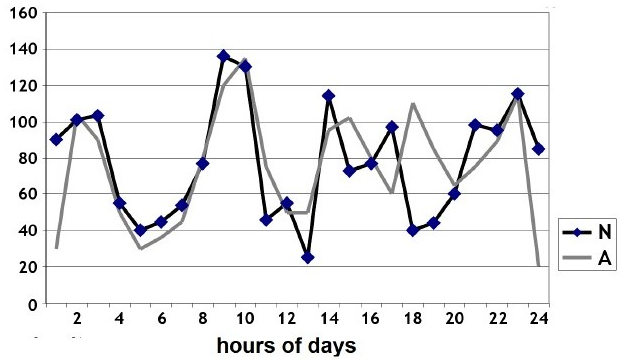
\includegraphics[width=70mm]{figs/ex-tsd.png}
% \end{center}
% 
% 
% \end{frame}


